\documentclass[10pt]{article}
\usepackage{tikz}
\usetikzlibrary{shapes.misc}
\usepackage[margin=0cm]{geometry}
\pagestyle{empty}
\tikzstyle{every node}=[cross out, draw, red]

\begin{document}

\vspace*{\fill}
\begin{center}
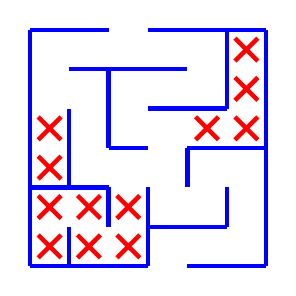
\begin{tikzpicture}[x=0.5cm, y=-0.5cm, ultra thick, blue]
% Walls
    \draw (0,0) -- (2,0);
    \draw (3,0) -- (6,0);
    \draw (1,1) -- (4,1);
    \draw (3,2) -- (5,2);
    \draw (2,3) -- (3,3);
    \draw (4,3) -- (6,3);
    \draw (0,4) -- (2,4);
    \draw (3,5) -- (5,5);
    \draw (0,6) -- (3,6);
    \draw (4,6) -- (6,6);
    \draw (0,0) -- (0,6);
    \draw (1,2) -- (1,4);
    \draw (1,5) -- (1,6);
    \draw (2,1) -- (2,3);
    \draw (2,4) -- (2,5);
    \draw (3,4) -- (3,6);
    \draw (4,3) -- (4,4);
    \draw (5,0) -- (5,2);
    \draw (5,4) -- (5,5);
    \draw (6,0) -- (6,6);
%Pillars
%Inner points in accessible cul-de-sacs
    \node at (5.5,0.5) {};
    \node at (5.5,1.5) {};
    \node at (0.5,2.5) {};
    \node at (4.5,2.5) {};
    \node at (5.5,2.5) {};
    \node at (0.5,3.5) {};
    \node at (0.5,4.5) {};
    \node at (1.5,4.5) {};
    \node at (2.5,4.5) {};
    \node at (0.5,5.5) {};
    \node at (1.5,5.5) {};
    \node at (2.5,5.5) {};
%Entry-exit paths without intersections
\end{tikzpicture}
\end{center}
\vspace*{\fill}

\end{document}
